\chapter{功能与结构设计}
本章节将给出Norm命令的基本功能以及全定制实现的总体结构图等。
\section{指令功能}
\indent  首先Norm指令具有如下形式:
\begin{center}
\textbf{NORM} (.unit)  $\quad$ \textit{src2, dst}
\end{center}
%{\centering  } 
其过程涉及两个操作数,\textit{src2}为输入操作数,\textit{dst}为目的操作数,位宽均为32位。需要实现的功能如下:
\begin{quote}
The number of bits of the first nonredundant sign bit from the MSB of the src2
operand is placed in dst.
\end{quote}

\indent 该指令的功能即根据符号位的数值统计前导零或一的数量,若符号位为1,则统计符号位后前导一的位数,否则统计符号位后前导零的位数。例子如图\ref{fig1.1}所示:
\begin{figure}[!hbpt]
\centering
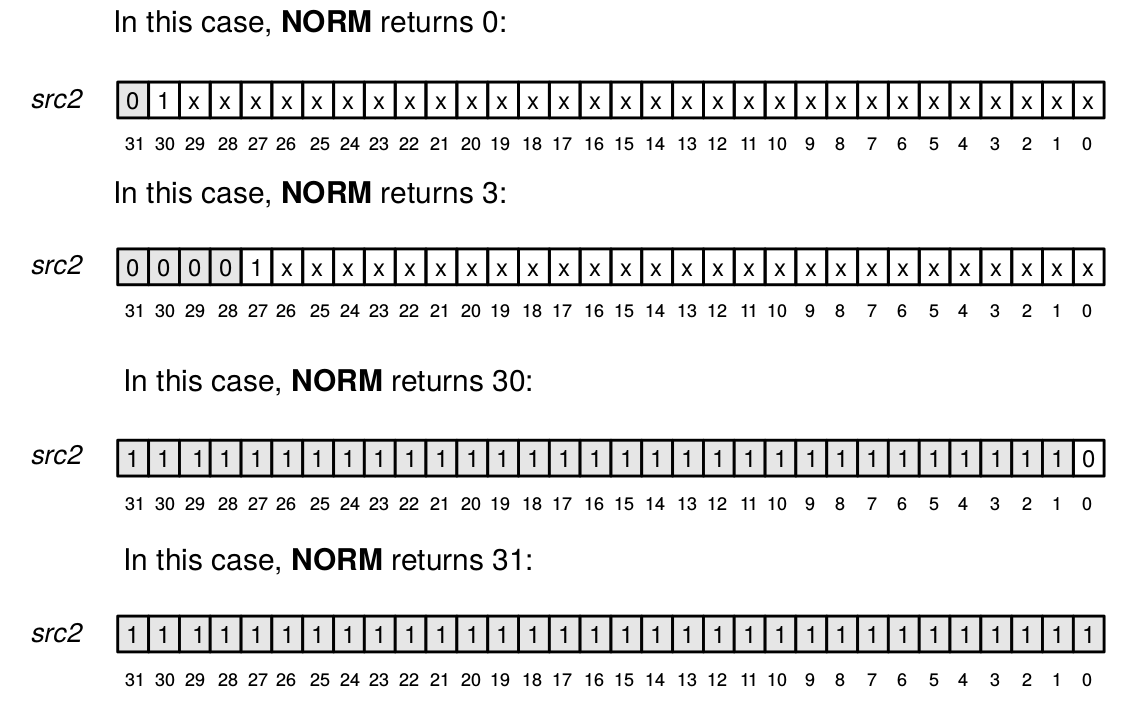
\includegraphics[width=0.8\textwidth]{chapter1/Norm_Example1}
\caption{NORM指令功能示例}
\label{fig1.1}
\end{figure}\\
并要求该指令需要在一个时钟周期以内完成运算。存在多种电路可以完成该指令的功能,但本次实验仅选择基于''前导零计数''的方式对其进行实现。
\section{设计思路及总体结构图}
本小节将给出NORM指令的设计思路,即各个子模块的原理,然后给出NORM指令的总体结构图。
\subsection{设计思路}
通过对上述指令的说明进行分析可以发现,该指令的功能为计算符号位后连续1或0的个数,连续零的个数可以通过前导零计算的模块进行,而前导1的个数可以通过先将输入操作数进行按位取反后再进行前导零的统计。
\subsubsection{前导零计算(LZC)模块}
通过以上讨论,可以明确前导零计数模块(LZC, Leading Zero Count Unit)的设计对NORM指令的实现至关重要。目前同样存在多种计算前导零的实现方法,文章\cite{dimitrakopoulos2008low}中给出了三种已有的计算方法,下面对其进行简单说明。在本章节的最后一部分中,给出该篇文章实现的低功耗改进方法,这也是本次实验采用的方案。
\begin{itemize}
\item \textbf{Encoder-Based LZC Unit}\\
第一种方法是基于两步编码过程的实现电路。首先检测Leading Digit(即前导零统计过程中的第一位不为零的位,前导1的统计过程中类似。),并将检测结果编码成One-Hot编码形式,如输入为00110100,则第一步的编码结果输入为00100000。为了得到One-Hot码,引入中间变量$S$,与One-Hot码不同的是,该中间变量在leading digit位之后的所有位都为1,例如同样输入00110100时,中间变量$S$为00111111。设$S$的第$i$位表示为$S_i, 0 \le i \le n-1 $,定义如下:
\begin{equation}\label{equ1.1}
S_i = A_{n-1} + A_{n-1} + \cdots + A_{i+1} + A_i
\end{equation}
其中$+$表示逻辑或运算。从公式\ref{equ1.1}可以看出$S_i$的含义为最高位与$i_th$位之间是否存在为1的位。在得到中间变量$S$后,通过将$S$的连续两位的数值来得到One-Hot码(用$L$表示):
\begin{equation}\label{equ1.2}
L_i = \overline{S}_{i + 1} \cdot S_i = \overline{S}_{i + 1} \cdot A_i \quad (0 \le i \le n-2)
\end{equation} 
其中$L_{n-1} = S_{n-1}$。得到One-Hot码$L$的电路被称为优先编码器(Priority Encoder)。

在本方法中用到的第二个编码器是将得到的One-Hot码转换为类似'' 8421''码的有权码。例如,对于输入为8位的数值的转换过程可以表示为:
\begin{equation}
\label{equ1.3}
\begin{gathered}
Z_2 = L_3 + L_2 + L_1 + L_0\\
Z_1 = L_5 + L_4 + L_1 + L_0 \\
Z_0 = L_6 + L_4 + L_2 + L_0
\end{gathered}
\end{equation}
经过上述两次编码后,即完成前导零统计的过程。

\item \textbf{Algorithm-Based LZC Unit} \\
已有的第二种计算前导零的电路被称为基于算法的统计。在该方法中,首先将输入$n$位数值分成$n/2$个连续两位构成的Groups.对于每一Group实行前导零计算。接下来,相邻的两个Group的计算结果被组合,且基于左Group的结果对两个结果进行选择。然后经过$\log_2n $次迭代后即可实现前导零检测的功能。这种方法可以通过模块化的方式进行全定制实现,同时也是目前已知的最快的基于静态CMOS的前导零实现方法。其示意图如图\ref{fig1.2}所示:
\begin{figure}[!hbtp]
\centering 
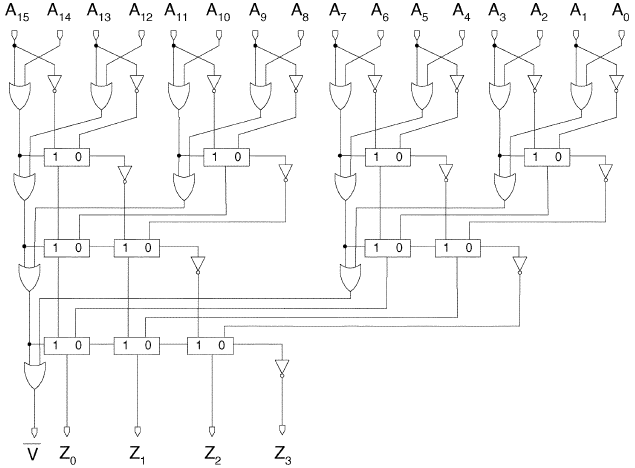
\includegraphics[width=0.9\textwidth]{chapter1/LZC_16bit}
\caption{Algorithm-based LZC的16-bit实现电路图}
\label{fig1.2}
\end{figure}
\item \textbf{Recursively-Based LZC Unit}\\
这种方法通过迭代的方式计算LZC结果(用$Z$表示)的第$i$位。下面以8-bit的LZC结算过程为例进行说明。首先对最高的4位进行$A_7A_6A_5A_4$检测,若此四位全为零,则说明输入的数值$A$中至少存在4个0,因此将$Z_2$置位,即得到$Z_2 = 1$,这意味着我们还需要对$A_3A_2A_1A_0$进行检测并统计。接下来则需要对$A_3,Z_2$以及$A_7,A_6$进行检测,并基于检测结果来决定$Z_1$的具体数值,并根据$Z_2$的数值来决定具体是根据$A_3,Z_2$还是$A_7,A_6$来确定$Z_1$的数值,然后重复上述过程,直至完成LZC统计。
\end{itemize}
\subsubsection{低功耗前导零计算模块原理}
在这一部分,将给出低功耗前导零计算模块的具体设计思路,即文章\cite{dimitrakopoulos2008low}中的''PROPOSED LZC ALGORITHM''一节。首先,将公式\ref{equ1.2}带入公式\ref{equ1.3}中可以得到如公式\ref{equ1.4}所示的结果:
\begin{equation}
\label{equ1.4}
\begin{gathered}
Z_2 = \overline{S}_4 \cdot S_3 + \overline{S}_3 \cdot S_3 + \overline{S}_2 \cdot S_1 + \overline{S}_1 \cdot S_0 \\
Z_2 = \overline{S}_6 \cdot S_5 + \overline{S}_5 \cdot S_4 + \overline{S}_2 \cdot S_1 + \overline{S}_1 \cdot S_0 \\
Z_2 = \overline{S}_7 \cdot S_6 + \overline{S}_5 \cdot S_4 + \overline{S}_3 \cdot S_2 + \overline{S}_1 \cdot S_0 
\end{gathered}
\end{equation}
通过对$S_i$的计算过程分析可以发现,$(S_i, S_j)\; with \; i > j$不可能取$(1, 0)$的结果,基于这一性质可以对$Z$的计算过程进行简化,最终可以得到如下结果:
\begin{equation}
\label{equ1.5}
\begin{gathered}
Z_2 = \overline{S}_4 \\
Z_2 = \overline{S}_6 \cdot S_4 + \overline{S}_2 \\
Z_2 = \overline{S}_7 \cdot S_6 + \overline{S}_5 \cdot S_4 + \overline{S}_3 \cdot S_2 + \overline{S}_1
\end{gathered}
\end{equation}
然后利用公式\ref{equ1.2}的关系将公式\ref{equ1.5}中的变量$S_i$替换为输入$A$,即得到公式所示的输入与输出的关系:
\begin{equation}
\label{equ1.6}
\begin{gathered}
Z_2 = A_7 + A_6 + A_5 + A_4 \\
Z_2 = A_7 + A_6 + \overline{A}_5 \cdot \overline{A}_4 \cdot (A_3 + A_2) \\
Z_2 = A_7 + \overline{A}_6 \cdot A_5 + \overline{A}_6 \cdot \overline{A}_4 \cdot A_3 + \overline{A}_6 \cdot \overline{A}_4 \cdot \overline{A}_2 \cdot A_1
\end{gathered}
\end{equation}
最后,文章\cite{dimitrakopoulos2008low}给出了统一的计算LZC结果每一位$Z_i$的公式:
\begin{multline}\label{equ1.7}
F(X_{n-1}, X_{n-2}, \dots , X_{1}, X_{0}) = X_{n-1} + \overline{X}_{n-2} \cdot X_{n-3} + \\
+ \overline{X}_{n-2} \cdot \overline{X}_{n-4} \cdot \overline{X}_{n-5} + \cdots + \overline{X}_{n-2} \cdot \overline{X}_{n-4} \cdot \overline{X}_{n-6} \cdots \overline{X}_2 \cdot X_1
\end{multline}
基于公式\ref{equ1.7}的8-bit LZC计算过程如图所示:
\begin{figure}[!hbtp]
\centering
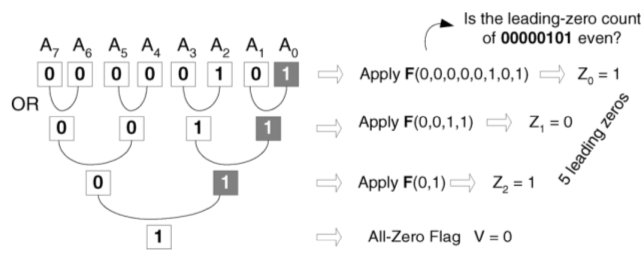
\includegraphics[width = 0.9\textwidth]{chapter1/LZC8bit}
\caption{8-bit输入LZC计算过程示意图}
\label{fig1.3}
\end{figure}
\subsubsection{低功耗16-bit LZC电路图}
基于公式\ref{equ1.7}的关系,可以得到16-bit输入时的LZC电路图,如图\ref{fig1.4a}所示,同时文章中还给出了一种功耗优化的改进电路,如图\ref{fig1.4b}所示。{\color{red} 可以看出,功耗优化后的电路图用到的器件数量更少,连线更加简单,且可以模块化实现,因此易于全定制设计,本次实验将采用图\ref{fig1.4b}的电路完成NORM指令的LZC子模块的设计。}
\begin{figure}[!hbtp]
\centering
\subfigure[16-bit LZC电路]{
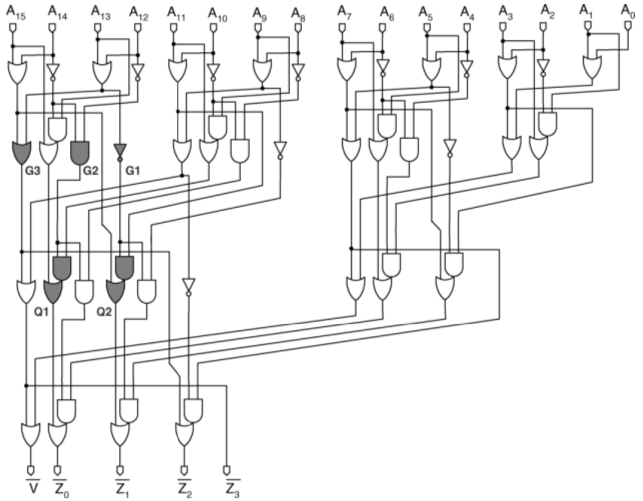
\includegraphics[width=0.45\textwidth]{chapter1/LZC16bit}
\label{fig1.4a}
}
\subfigure[功耗优化的16-bit LZC电路]{
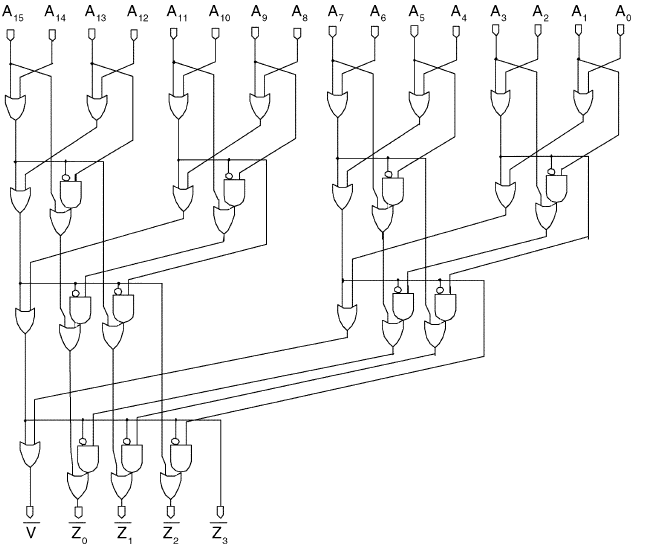
\includegraphics[width=0.45\textwidth]{chapter1/NewLZC16bit}
\label{fig1.4b}
}
\caption{16-bit的LZC电路及其功耗优化电路}
\label{fig1.4}
\end{figure}

关于低功耗LZC的设计更详细的信息可参考文章\cite{dimitrakopoulos2008low}。
\subsubsection{2路31位选择器的设计}
由于NORM指令除了需要检测前导零,还需要完成前导一的检测,因此,在设计过程中将输入的32位数据分成两路,一路将$0 \sim 31$位进行取反,另一路不做处理,并根据符号位是0还是1进行选择,即若符号位为1,则选择取反后的数据送入LZC电路,若符号位为0,则将不做处理的数据送入LZC电路。2路31位选择器的每一位基于图\ref{equ1.5}所示的1位选择器实现:
\begin{figure}[!hbtp]
\centering
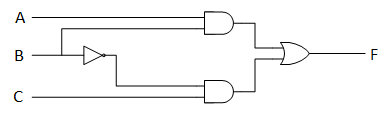
\includegraphics[width=0.9\textwidth]{chapter1/MUX2_1}
\caption{2路1位选择器单元}
\label{fig1.5}
\end{figure}\\
\noindent 其中,若$B$为0,则F为C端输入的数据,若$B$为1,则F为A端输入的数据。
\subsection{总体结构图}
基于以上讨论,可以得到NORM指令的总体结构图,如图\ref{equ1.6}所示。
\begin{figure}[!hbtp]
\centering
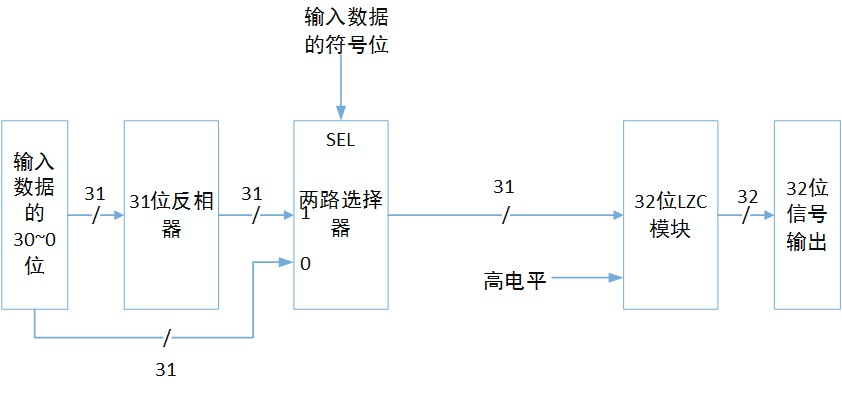
\includegraphics[width=0.9\textwidth]{chapter1/NORM}
\caption{NORM指令结构框图}
\label{fig1.6}
\end{figure}
\section{算法流程}
本小节将结合图\ref{equ1.6}对NORM指令的实现过程进行详细说明。

首先,输入数据的位宽为32位,由于NORM指令不仅需要计算符号位后连续0的个数,而且还要计算符号位后连续1的个数,因此为了实现电路复用,,选择将输入数据的$30 \sim 0$位数据分成两路,一路按位取反,一路不做任何处理,然后将31位反向器的结果与原始数据送入两路31位选择器,选择信号为输入数据的符号位,其工作原理为:若符号位为1则选择反向器的结果,否则选择原始数据。两路选择器的结果接下来被送往32位LZC模块,该模块实现前导零计算的功能。由于LZC是32位而输入数据是31位,因此还需要额外的一位数据输入到32位LZC中,且输入的数据不能影响NORM指令的正确性,因此在这里LZC的最低位的输入被设置为恒1。最后,将32位LZC的结果输出,此即为NORM指令的结果。
